% Section 5 in file hwsw.tex

% Section 5.1
\subsection{Radio Transceiver}
For the radio transceiver of WHCS the chip that we decided to use is Nordic
Semiconductor{}'s NRF24L01+. This chip meets all the requirements that we set
for our radio transceiver. The NRF is also a very popular chip that is easy to
find and rarely out of stock. This is a benefit to the manufacturability of
WHCS because NRFs are cheap and easy to buy in bulk. Alternatively we could
have chosen to use an XBee radio device which implements the zigbee 802.15.4
IEEE standard, however we did not see the need for this. XBee devices are also
more expensive than the NRF chips that we have decided to utilize.

% Section 5.1.1
\subsubsection{Operating Principles and Usability of NRF24L01+}
The NRF24L01+ is a radio transceiver that operates in the ISM (Industrial,
Scientific, and Medical) radio band. The range of channels for the NRF is
2.4GHz to 2.527 GHz, however because the designated ISM band that we are using
only ranges from 2.4GHz to 2.5GHz we will not be able to use all of the NRF{}'s
available channels. With the NRF we are capable of sending payloads with a
maximum size of 32 bytes per transmission from module to module. We will be
able to change the data length from 1 to 32 bytes in order to find the optimal
mix between reliability and speed. Every NRF chip has the ability to
simultaneously store 1 transmission address and 6 receiving addresses. The
first receiving address is utilized if the auto{}-acknowledgement feature is
enabled, so effectively there are 5 receiving addresses.  This capability gives
us flexibility for implementing our network because we make decisions such as
having a dedicated address to each node in the network as well as an address
for broadcasts of certain types. The addresses of the NRF are 5 bytes wide so
we will be able to have many NRF modules within the network. A very useful
feature of the NRF is the ability to enable auto{}-acknowledgement. When this
feature is activated the receipt of a transmission from one NRF to the other is
auto{}-acked without the need from any upper level software. This simplifies
the work necessary for creating our own network of NRF chips. We will be able
to confirm the receipt of data therefore increasing reliability.  This
auto{}-ack also allows the NRF to perform retries up to a given limit, so just
in case there is noise during the transmission the NRF will repeatedly try to
transmit again. The NRF also allows for low power mode and long range mode.
For WHCS we will be able to tweak whether or not to use long range mode or not
depending on the performance of the system within its environment.

The NRF requires 3.3v of electricity to operate so all parts of WHCS will
require a 3.3v line. The datasheet lists the current consumption while in
receive mode as 18mA. This will be the most common mode for the NRF chips
present in WHCS so they can be ready to receive commands at any time. The chip
receives commands from a microcontroller through SPI (Serial Peripheral
Interface). This is great because the NRF design philosophy fits perfectly with
our microcontroller based base station and control modules. Beside the standard
MOSI, MISO, and SCK for SPI, the NRF also has a csn pin for telling it to
receive commands, ce pin for telling to to transmit or receive at that moment,
and an interrupt pin for notifying the microcontroller of important situations.
The csn pin will allow the SPI bus to be shared with other components such as
the LCD being used for the base station. The interrupt wire pin can be
monitored in order to listen for data received, data sent, and data failed to
send notifications. In total the NRF will take up 6 pins whilst three of the
pins will be shareable with other SPI components.

% Section 5.1.2
\subsubsection{Driver Use Case}
The NRF chip that we have decided to use for communication in WHCS will need to
have a driver written for it. This will help keep the way we interface with the
NRF consistent and will provide clean code. All of the network code that we
write for the base station and the control modules will be relying on the
integrity of the NRF driver that we write.  The driver provides the foundation
and if it is not reliable then none of the code we write for our system will be
reliable. The focus for the development of the NRF driver is elegance. We want
everything the NRF driver offers to be simple yet accomplish everything
necessary. We have developed the use case diagram pictured in
\autoref{fig:nrf-usecase-diagram} as a guideline for the development of the NRF
driver. The NRF driver should provide the functionality included in the use
case diagram in an easy to use format.  These will be the most common uses of
the NRF.

\ucfgfx[scale=0.4]{fig:nrf-usecase-diagram}{a51-img001.png}{NRF Driver Use-case Diagram}

The core use of the NRF driver is transmitting and receiving payloads. Every
other use case is a supporting role for the final goal of transmission. The
basis of the driver will be reading and writing registers. Everything will
build off of this capability, especially reading and writing the payload for
transmission. Other use cases such as changing power mode, checking the status
of the chip, and changing from a transmitter to a receiver will be special
forms of writing to a register. Thus reading and writing to registers is a use
of the driver, however it will be abstracted in a way that provides ease of
use. A user of the NRF driver will spend most of the time setting addresses,
writing payloads, transmitting payloads, and analyzing interrupts. These use
cases need to be implemented perfectly to provide a strong foundation for the
networking of WHCS.

% Section 5.1.3
\subsubsection{Driver Class Diagram}
It was decided that the best design approach for implementing the NRF driver
was as a class in C++. We will be using atmega microcontrollers in WHCS so C++
is supported as a development language. Using C++ allows us to create a class
that can leverage object oriented programming techniques such as encapsulation.
The class diagram for the driver is shown in \autoref{fig:nrf-class-diagram}.
Primitive functions such as ReadByte and WriteByte can be hidden from a user
while PowerUp will be exposed as a public function. Using C++ also gives us the
ability to use a constructor when using the WHCSNrf class, and in this
constructor we can assign the only thing varying between uses of the NRF, the
chip enable pin and the chip select not pin. Assigning the ce pin and the csn
pin are the first step of using the NRF driver. Any communication between the
microcontroller and the NRF will rely on the proper assignment of these pins.

%\begin{wrapfigure}{r}{0.5\textwidth}
%  \begin{center}
%      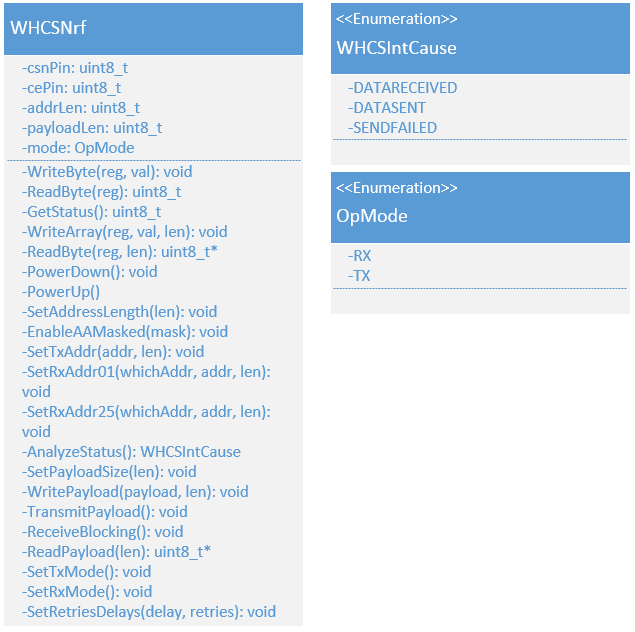
\includegraphics[width=0.48\textwidth]{a51-img002.png}
%  \end{center}
%  \caption{NRF Class Diagram}
%  \label{fig:nrf-class-diagram}
%\end{wrapfigure}
\ucfgfx[scale=0.5]{fig:nrf-class-diagram}{a51-img002.png}{NRF Class Diagram}

Usage of the NRF driver will involve first constructing the class by telling
the microcontroller which pins the NRF is connected to. Then the user will be
doing everything necessary to customize the way that data is transmitted and
received. The driver exposes the common settings in an easy to access manner.
Enabling things such as auto{}-acknowledgement and the number of retries for
the transceiver can be done with the call of a function with simple parameters.
Setting the address for receiving and transmitting data can be done in one line
of code. The SetTxAddr function will be one of the most utilized function for
an NRF involved in a network constantly sending payloads to other chips. A
typical use will involve powering up the NRF with the PowerUp call, setting the
transmission address, writing a payload, and then transmitting a payload. With
this driver, the user does not need to know the registers involved with the
NRF. The hardware interactions with the chip are all abstracted away.

% Section 5.1.4
\subsubsection{Network Library}
\label{sec:network-library}
\todo{3 pages}

% Section 5.2
\subsection{Microcontrollers}
\todo{Talk about pin count and having to disable the JTAG fuses to get access to those pins}
\todo{Talk about the speed grade for the CPU and why a higher grade would be faster}

For the proper operation of WHCS microcontrollers will need to be installed
into all of the control modules as well as the base station. This meant
research was needed to choose what the best microcontroller for each of the
modules was.  The base station is a bit more hefty than the control modules so
the design considerations are different for the two.  The first step was to
figure out what family of microcontrollers to use.

% Section 5.2.1
\subsubsection{Microcontroller Brand}
Choosing the microcontroller brand would set the path for all the development
that we do with the microcontroller. Every other choice would stem from this
decision so we wanted to make a smart choice. We weighed out the documentation,
support, ease of acquisition, ease of use, and community for the brands that we
considered. Our initial choice was Texas Instruments because of the use of the
MSP430 launchpad board in the UCF curriculum. The fact that using the MSP430
was required in EEL 4742 (Embedded Systems) meant that everyone was already at
least somewhat familiar with it.  The familiarity factor was a plus for the
MSP, and we all knew that T.I. has very good, albeit lengthy, documentation for
their chips. A quick look at digikey showed that MSP430 microcontroller chips
were well in stock so there would be no problem acquiring them if they were the
chip that we wanted to use. The thing that we were unsure about with using
Texas Instruments chips was the community surrounding the brand. For example if
we encountered a problem rewriting a fuse on the microcontroller would we be
able to find a forum of people who knew how to solve the problem, and things of
that nature.

While we researched Texas Instruments based microcontrollers we also researched
the Atmel brand. We knew Atmel is very popular especially because they produce
the chip used on the Arduino development boards. We checked how the Atmel chips
were documented by looking at the datasheet for the Atmega 88, and were pleased
with how well things were laid out.  Digikey had most of the common brands of
Atmel chips in stock so acquisition would be no problem. We didn{}'t feel the
need to consider any other brands because we felt that between the two choices
we looked into they could both suit our needs. Atmel offered chips and brand
support similar to that of Texas Instruments, so for whatever kind of chip we
required we could use Atmel or T.I. For us the choice came down to how
prominent the communities for the two brands are. Ultimately we decided that
the Atmel brand had a very pervasive community that was sure to aid us in our
utilization of any chips produced by the company. While the MSP430 was familiar
to all of us the Texas Instruments chips did not seem as broadly used across
the open source populus. So our final decision was to use the Atmel brand of
microcontrollers for WHCS.

\subsubsection{Base Station Microcontroller}
The base station is the center of operations for WHCS so it needs the most
computing power. It has the most data structures to take care of, the most
commands to process, and the longest compiled program. The microcontroller for
the base station also needs to be able to connect to the LCD screen, the radio
transceiver, and BlueTooth transceiver all at the same time. So taking all
these things into consideration for choosing the microcontroller was important.
We needed a large amount of pins to interface with all the peripherals,
especially because we knew we wanted a parallel interface LCD. A large amount
of flash memory was also a trait that we looked for since we knew the base
station would be doing a lot, thus making its program long. The first big
decision was whether to use an ARM based microcontroller for our base station
since it was the brains of the system. ARM microcontrollers have much higher
processing power, but also introduce complexity. Many ARM microcontrollers
don{}'t have on board flash memory so that is an added layer of design that is
needed to get the unit working. After considering the processing necessary in
the base station and the bandwidth of the network in WHCS we realized that an
ARM based microcontroller would not be necessary. There was not enough data to
be processed to warrant the use of an ARM microcontroller. Using an ARM unit
would introduce design complexity for a solution that could be attained through
easier means.

Eventually our research efforts landed us upon the Atmega series of Atmel
microcontrollers. These microcontrollers are often thought of as the flagship
Atmel chips in the DIY community and they did seem highly capable. The chips
were cheap, had plenty of pins, plenty of on{}-chip peripheral support such as
the UART, were easy to program, and were highly available. After browsing the
Atmega series of chips we narrowed down the chip that we would be using for the
base station to the three chips listed in \autoref{tab:atmega-chips}. The table
shows that the lowest maximum operating frequency between the three is 16 MHz
which is more than capable of powering the low bandwidth network of WHCS. 16
MHz is enough to handle communication, the LCD display and interrupt vectors,
so all the chips are viable options in that feature. The 8 KB of flash memory
was low compared to the 32 KB offered by the other two so we actually took that
chip out of the running when we considered that the base station would have a
large routine. When we were down to choosing between the Atmega328 and the
Atmega32A we realized that the Atmega32A was actually the only option between
the two chips that would work. The reason for this was the number of I/O pins.
We had picked the LCD, radio transceiver, and BlueTooth chip that we would be
using and the Atmega32A was the only chip with enough I/O pins to support all
the peripherals. Our final decision was to use the Atmega32A as the
microcontroller for the base station.

\begin{table}[H]
\centering
\begin{tabular}{|l|l|l|l|}
\hline
{\color{black} Atmega MCU} &
{\color{black} Flash Memory (KB)} &
{\color{black} Max I/O Pins} &
{\color{black} Max freq. (MHz)}\\\hline
{\color{black} Atmega88} &
{\color{black} 8} &
{\color{black} 23} &
{\color{black} 20}\\\hline
{\color{black} Atmega328} &
{\color{black} 32} &
{\color{black} 23} &
{\color{black} 20}\\\hline
{\color{black} Atmega32A} &
{\color{black} 32} &
{\color{black} 32} &
{\color{black} 16}\\\hline
\end{tabular}
\caption{comparison of ATMega chips}
\label{tab:atmega-chips}
\end{table}

After we had decided to use the Atmega32A as the microcontroller for the base
station there were still some things that needed researching to make it usable.
The main issue was disabling the JTAG interface on port C to make the pins
usable as general I/O. After researching the data sheet and the community
forums we found that to be able to use port C pins as GPIO the JTAG fuse must
be disabled. Otherwise setting these pins on port C to high or low will have no
effect.

\subsubsection{Control Module}

\subsubsection{Development Environment}

\subsubsection{Programming}

\subsubsection{External Oscillator}

\subsection{BlueTooth Chip}
The BlueTooth device for WHCS will enable the base station to communicate with
the mobile phone controller. Our guidelines for choosing a BlueTooth device
included ease of use, reliability, size, cost, availability, and documentation.
There were a multitude of BlueTooth devices to choose from. Special attention
was paid to how well the BlueTooth device could connect to a microcontroller
UART. Two BlueTooth devices, the HC{}-05 and the RN{}-41, showed the most
promise. Our research of the two devices showed that they both had their
advantages and either one could be implemented in our design. After careful
consideration we chose to utilize the HC{}-05 in our design, however the
RN{}-41 could still replace the HC{}-05 if necessary.

An important factor for considering the BlueTooth devices was if the internal
settings of the BlueTooth devices could be changed and if possible how. Such
internal settings include things such as the device{}'s BlueTooth name, baud
rate, and passcode. These things need to be changed from their default settings
or else many BlueTooth devices would have similar names, and they would all
have default passcodes. We want to implement good security into WHCS so we need
to be able to change the default passcode for the BlueTooth device. Also the
baud rate is usually low in BlueTooth devices by default, which can be bumped
up depending on the microcontroller being used. A BlueTooth device that could
not be programmed manageably was not an option.

% Section 5.3.1
\subsubsection{RN-41}
The RN{}-41 is a BlueTooth module designed by Microchip. This module is
designed to be an all inclusive solution for embedded BlueTooth. It is clear
that a lot of design went into this chip because it is very high quality and
the data sheet is very thorough. Along with the high quality of the module
comes the high cost. Of the two considered BlueTooth modules the RN{}-41 was
much more expensive with a price of \$21.74 from Microchip. The high price tag
makes it a less appealing option out of the BlueTooth devices because they are
effectively accomplishing the same thing. The module itself appears well
designed visually and it has dimensions of 25.8x13.2mm so it is not obtrusive
and could fit well onto a PCB. There are 24 pins on this device and the
datasheet gives the dimensions down to the pin spacing allowing for easy PCB
layout design. The RN{}-41 makes communicating with microcontroller UARTs easy
by simplifying RS{}-232 down to the Rx and Tx wires. This means the only
connections necessary for using the RN{}-41 with a microcontroller are power,
ground, Rx, and Tx. The microcontroller{}'s that we have decided to use include
Rx and Tx pins that hook up directly to the RN{}-41. From the
microcontroller{}'s point of view the BlueTooth device does not even exist. The
RN{}-41 acts as a transparent man{}-in{}-the middle and simply relays messages
from a BlueTooth device to the microcontroller and vice versa. This is perfect
for our design because the RN{}-41 could just be plug and play. With an
advertised 100 meter transmission range the RN{}-41 meets the requirements we
set for distance of BlueTooth reception.  According to the datasheet the
RN{}-41 has a maximum baud rate of 921K which means it goes above and beyond
the transmission rates necessary for communicating between the mobile device
and the base station.

The RN{}-41 has a manageable means of programming the internal settings. When
the RN{}-41 is on, sending {}``\$\$\$'' over the UART lines puts the chip into
command mode. From here there are a list of commands that can be passed in
order to inquire or manipulate the state of the module. There are advantages
and disadvantages to this approach. It is great that it is easy to program the
RN{}-41 just by passing certain data while it is wired normally, however in the
event that the sequence {}``\$\$\$'' was ever passed during operation it could
throw off the whole system. This is not a terrible thing but it is worthy of
consideration.

% Section 5.3.2
\subsubsection{HC-05}
The HC{}-05 is a BlueTooth module that shares many similarities with the
RN{}-41. It is of comparable size to the RN{}-41 with dimensions of 27x13mm.
HC{}-05 modules are also commonly sold along with a breakout board with male
headers. This makes it an option to have the PCB include female headers and use
them for installing the HC{}-05. Our intention for the base station containing
the BlueTooth module is to have the PCB board hidden, so using female headers
for plugging in the HC{}-05 to the PCB is a viable option. The module is
advertised as a low power class 2 BlueTooth device with power consumption for
communication listed at 8 mA. This is lower power consumption than the RN{}-41.
The max signal range is not listed in the data sheet, however we have tested
this chip and have achieved a signal range of more than 50m which is more than
enough for what we desired in our BlueTooth chip. Just like the RN{}-41 the
HC{}-05 communicates to microcontrollers by simplifying RS{}-232 and only using
the Rx and Tx pin. The maximum supported baud rate is 460800 which will allow
for very fast data transfer and will exceed the needs of communication speeds
in our system.

The HC{}-05 comes with default settings similar to most BlueTooth modules. The
default baud rate is 9600 and the default passcode is 1234. In order to change
this the module must be accessed in AT mode. AT mode is entered by utilizing
pin 11 {}``key{}'' on the HC{}-05. When this pin is held high, the module
enters AT mode on startup and is ready to take commands. This means that
whenever we want to program the BlueTooth module we will need to use a
microcontroller with a UART connection to a terminal as well as a UART
connection to the HC{}-05. This will require the implementation of a software
Rx and Tx pin. This will only need to be done once because once the BlueTooth
module has been programmed it retains that configuration. The requirement of
holding the key pin high during startup of the module eliminates the danger of
entering the programming mode during normal operation.

For WHCS we have decided to use the HC{}-05 as our BlueTooth module instead of
the RN{}-41. \autoref{tab:bluetooth-compare} shows highlights of the features of each
BlueTooth module that led to the decision. The main factors deciding this were
the cheaper price of the HC{}-05 and the fact that they both accomplish the
same thing. The table shows clearly that the HC{}-05 is a much more affordable
option. The two chips were comparable in size, features, wiring, layout, and
usability however at the price of \$6.64 the HC{}-05 cost less than half of the
RN{}-41. The RN{}-41 is the second best choice and can serve as a fallback if
HC{}-05 chips went out of stock or an unforeseen circumstance occurred.

\begin{table}[H]
\begin{tabular}{|l|l|l|l|l|l|}
\hline
 &
{\bfseries Cost} &
{\bfseries Range (meters)} &
{\bfseries Breakout Option} &
{\bfseries Configurable} &
{\bfseries Size}\\\hline
{\color{black} RN{}-41} &
{\color{black} \$21.70} &
{\color{black} 100} &
{\color{black} No} &
{\color{black} Yes} &
{\color{black} 25.8x13.2mm}\\\hline
{\color{black} HC{}-05} &
{\color{black} \$6.64} &
{\color{black} 50+} &
{\color{black} Yes} &
{\color{black} Yes} &
{\color{black} 27x13mm}\\\hline
\end{tabular}
\caption{comparison of the BlueTooth chips}
\label{tab:bluetooth-compare}
\end{table}

% Section 5.4
\subsection{LCD}
\todo{whole section}
Being able to interface with WHCS like a normal wall thermostat is one of our
project goals. Having a centralized display that can quickly display the most
important information for homeowners would be step up from traditional ``dumb''
thermostats. With a simple LCD combined with a touchscreen, users would have a
way to control and query their home without having to find their phone.

To make this a reality, we have chosen the versatile, premade, and well
supported Adafruit 2.8" TFT LCD\footnotemark{} with a resistive touchscreen.
Internally, the display is driven by the feature-rich
\href{http://www.newhavendisplay.com/app_notes/ILI9341.pdf}{ILI9341 chipset}.
This chip is specifically created for a 240x320 pixel LCD with a focus on
small, power-conscious mobile devices. Another reason we chose to buy this from
Adafruit and not integrate the chip directly is due to the complexity of the
design. Also, with the abstracted product, there are
\href{https://github.com/adafruit/Adafruit_ILI9341/tree/master/examples}{plenty
of usage examples} and Adafruit's
\href{https://learn.adafruit.com/adafruit-2-dot-8-color-tft-touchscreen-breakout-v2}{excellent
technical documentation}. This combined with Adafruit's
\href{https://github.com/adafruit/Adafruit_ILI9341}{libraries}, assure
that integrating the LCD will be straight forward. The one issue with
this solution is with the ILI9341 driver code: it was written to target the
Arduino platform. Now, the Arduino platform is fairly close to bare AVR, minus
the remapped pin numbers and some support libraries, so porting Adafruit's library
would be a feasible solution. Our plan is to use the existing driver along with the chip datasheet to create a library specific to our needs. That way we get full control over the port placement and the experience of creating an LCD driver.

\footnotetext{\url{https://www.adafruit.com/products/1770}}

% Section 5.4.1
\subsubsection{Capabilities}
\todo{1 page}
In terms of capabilities, we have summarized the main features of the LCD module in \autoref{tab:lcd-features}

\begin{table}[H]
\centering
\begin{tabular}{|l|l|}
\hline
\bfseries Specification & \bfseries Description \\ \hline
Resolution & 240x360 \\ \hline
Colors & 262K @ 18bits, 65K @ 16bits \\ \hline
Voltage Input & 3.3 - 5V \\ \hline
Weight & 40 grams \\ \hline
Dimensions (LCD itself) & 2.8" diagonal \\ \hline
MCU Interface & Multiple. See \autoref{sec:lcd-driver}\\ \hline
Touchscreen technology & Resistive (one finger)\\
\hline
\end{tabular}
\caption{a brief summary of the pertinent features of the LCD module}
\label{tab:lcd-features}
\end{table}

These features are more than sufficient for out application as most of the
drawing we will be doing will be non-realtime. Nearly all of the displayed
information will be text and UI element, which don't change often. For an
overview of our UI elements, see \autoref{sec:ui-lib}.

One of the beneficial features of the LCD is that it gives developers a choice
of which interface to use. The broken out interfaces are 4-bit SPI and 8-bit
parallel. For prototyping, we used the low pin count SPI interface, but for our
final design, we will be using the 8-bit interface to avoid having to wait for
lengthy SPI transfers. Also, our NRF radio will be using the SPI bus, which
should have priority over that channel.

\missingfigure{LCD Pinout}

Another feature of Adafruit's module is the resistive touchscreen present on top of the
LCD. With this, we don't just have to display information about WHCS, we can
receive commands as well! Using this simple interface, we plan on creating a
featureful UI library to communicate up-to-date information about the home
while allowing for user control. The specific interface for the touchscreen
requires 4 pins, 2 of which must be connected to the MCU's Analog to Digital
Converter. By reading the resistance of the touchscreen, we would be able to
calculate the position of a single finger.

Finally, one extra component on the LCD module is an SD card slot. We are free
to read and write directly to this card to store large images, such as logos
for display on the LCD. We plan on storing at least our logo, but we may also
store fancy UI badges such as arrows ($\leftarrow,\rightarrow$), X's
($\otimes$), checkboxes (
\makebox[0pt][l]{$\square$}\raisebox{.15ex}{\hspace{0.1em}$\checkmark$}), and
anything else we can think of.

\subsubsection{ILI9341 Driver}
\label{sec:lcd-driver}
\todo{2 page}

In order to perform the required operations for drawing pixels to the LCD, we
need a robust driver to manage the state of the ILI9341 chip. This driver will
have to have primitives for choosing a position to draw and the ability to fill
pixels.


\missingfigure{class diagram}

\subsubsection{Touchscreen Driver}
\todo{1 page}
The touchscreen will need code dedicated 

\missingfigure{diagram showing the touchscreen coordinates}

X+, X-, Y+, Y-

\subsubsection{Graphics Driver}
Unlike the previous ILI9341 driver, our graphics driver will be in charge of
taking the low-level primitives exported by the LCD driver and using them to
draw useful screen elements. These include text, lines, rectangles, circles,
and images. The driver will essentially contain a set of routines for drawing
these objects given a set of parameters such as length/width for rectangles,
radius and position for circles, and bitmap lookup-tables for the text. These
functions and more are already created by Adafruit, but for the experience and
control of designing the graphics routines, we choose to implement our own.

Due to the unique hardware and software constraints (i.e limited clock speed
and memory), we must take care to not exceed the capabilities of the hardware.
This means floating point operations, which may be required for shapes such as
a circle must be optimized or not used at all. A quick optimization for
floating point operations would be to use a $sin()$ lookup table and only
integer multiplications. These performance issues will be addressed as needed
and only if necessary. By avoiding unnecessary optimizations, we will save
valuable time for building out the library.

\paragraph{Algorithms Necessary}
The functionality of graphics driver depends on some core algorithms for
efficiently creating meaningful screen objects. One of these core algorithms is
\href{https://en.wikipedia.org/wiki/Bresenham\%27s_line_algorithm}{Bresenham's
line algorithm}. This algorithm needs to be efficiently implemented as it will
be the base for nearly every derived graphics operation. For example, a
transparent rectangle has four sides which results in four calls to this line
drawing function.

\paragraph{Character Lookup Table}
In order to convey useful information, we will need to display text to the
user. This text will be stored in an effcient lookup table for quick drawing
operations similiar to \autoref{fig:character-lut}. On a limited embedded
system like this, there is a limited amount of time that can be dedictated for
font rendering. To save on time, we will use an existing font available online.
Adafruit also bundles a font in with their graphics library that is implemented
as a function instead of a block of memory.

\ucfgfx[scale=0.5]{fig:character-lut}{raster-character}{a raster image showing
a possible character lookup table}

\subsubsection{UI Library}
\label{sec:ui-lib}
\todo{2 page}

%\begin{itemize}
%\item line drawing algorithms
%\item wow
%\end{itemize}

% Section 5.5
\subsection{Android Application} For most WHCS users the mobile application
will be the only physical interaction they have with the application. When we
set out for development we wanted to make an easy to use application that would
attract users to stick with our system.  Operability and usability were
emphasized in our design process. We wanted an appealing U.I. without
complexity, after all we are targeting a simple solution to home automation.

% Section 5.5.1
\subsubsection{Development Environment} Android is the mobile operating system
that we chose to utilize for our BlueTooth enabled phone. The Android operating
system is accessed through the Java language, which is a staple in the UCF
curriculum therefore everyone in our group is versed in it. Developing on
Android is also a free endeavour where as developing on an iPhone requires
enrolling in the Apple Developer Program. These programs actually cost a good
amount of money that is unnecessary to spend. The Windows Phone platform is
another option for the BlueTooth enabled phone, but they are very unpopular so
we chose not to target this platform. With our target narrowed down to the
Android operating system, we had to research what the best environment for
developing our application would be. There were three options that we
considered for managing the Android project each with their own perks: command
line tools, Eclipse, and Android Studio.

The first development environment we considered for our Android project was
creating our own project structure and using command line build tools. There
are also debug tools available on the command line for Android projects. These
tools would be necessary in order to do our testing on Android Virtual Machines
running on our computers. This approach favors people who are command line or
terminal oriented. Linux is popular within our group and the ability to do
things from the terminal is appealing so this approach seemed like a good one.
We realized that with the design we had in mind for our project, it would
become quite large and it might be difficult to handle without a dedicated IDE
(Interactive Development Environment). This led us to looking into using
Eclipse for developing our Android application. Eclipse seemed like a natural
choice because it is what is recommended for using in the Java oriented UCF
programming classes.  The Android SDK provides an add{}-on for Eclipse that
makes it a viable Android development environment. We were able to get this
running and create sample Android applications. Inside of Eclipse the project
structure for Android applications is laid out nicely. The debug tools are all
organized at the top of the screen resulting in an easier development
experience than debugging from the command line. The problem with using Eclipse
as our IDE is that Eclipse is notorious for being slow and unwieldy.

\color{black} Recently Google released a development environment named Android
Studio that is made specifically for developing Android Applications. No one in
our group had any prior experience using this IDE, however we realized that due
to it being tailored specifically for Android it was probably better than
anything else. This turned out to be correct, because it was much easier for us
to create an Android project and navigate our code from within this IDE. We
also decided to use Android Studio because it has built in Git support for
source control. \autoref{fig:git-scm} shows the important feature offered by
Android Studio that we use for collaboration. This meant that as we were
writing our code we could easily submit our changes to a remote Git repository.

\ucfgfx[scale=0.7]{fig:git-scm}{a55-img001.png}{Git source control in Android Studio}

\subsubsection{Use Case Diagram} The central use cases for WHCS are toggling
the state of certain devices within the home and monitoring certain states.
For example a user of WHCS will spend most of the time turning on lights,
checking whether a light is on, or checking the temperature reading of a
certain sensor. There are certain other use cases that are necessary in order
for WHCS to be a functioning application, as well as to make it have a robust
feel. Features like speech activation and creating endpoint groups are
usability features that are not necessary in order to accomplish the central
goals of WHCS.  Connecting to the base station the first time you use the
application is a necessary use case that must be incorporated into the
application. \autoref{fig:android-usecase} shows the use case diagram for the
WHCS application.

The design for the WHCS application involves making sure that performing the
common use cases such as checking status and toggling endpoints are very fast.
The user should be able to perform these tasks without having any knowledge of
how the application works. Speech recognition will be a supporting feature so
it does not need to be a central focus like the area that will visualize the
control modules. When the user wants to perform speech activation it will
involve pressing a button to prompt the speech recognizer, and then giving a
command to the WHCS. In order to make the speech activation feature more
promising, the user will have the ability to rename endpoints for activation.
Creating endpoint groups will be a feature that is not used frequently but adds
a lot of value to the application. Users will only have to create an endpoint
group once for it to last in the application. Creating an endpoint group will
be a simple task involving assigning a group number to endpoints. That number
will be the endpoint group, then that endpoint groups state can be toggled.

\ucfgfx[scale=0.45]{fig:android-usecase}{a55-img002.png}{Android App Use-case diagram}

\subsubsection{Speech Recognition} The Android application for WHCS will offer
speech activation capabilities. These will be on top of GUI activation
capabilities. The speech activation sequence begins with the press of a button
to start the speech recognition. The user will be prompted with a microphone
and can then give his command. The commands will be formatted like {}``light
one on.'' When the user gives commands using the speech method, a notification
will be given indicating the success of interpreting the speech into a known
command. If the user{}'s speech does not match a known command, the speech will
be shown back to the user to show what went wrong. We are predicting that the
most frequent cause of this will be the Android phone mishearing the user. In
the event that the speech matches a command, the application will display the
command to the user and then perform it. The following flow chart in
\autoref{fig:android-speech} displays the sequence of events happening when a
user performs speech activation.

\ucfgfx[scale=0.4]{fig:android-speech}{a55-img003.png}{Android app speech activation
chart}

The goal of the speech activation feature is to be easy to use. In order to
promote the usage of this feature we will add the ability for users to rename
the endpoints that the speech commands will target. For example the user could
change {}``light 1'' into {}``living room light.'' This way the user could say
{}``living room light on{}'' to the application in order to turn on the living
room light. To do this data structures will need to be stored in the
application which hold the preferred name of each type of endpoint. Endpoints
can be distinguished by the type they are, their individual identifier number
and their preferred name. The preferred name should be stored when the
application is closed so a permanent source of storage is needed to do this.
The file system can be used or possibly a sqlite database.

In the code for our application we will be using the Android speech recognition
API (Application Program Interface).  Android has a speech recognition service
that can be started by requesting it within an application. We will request
this service to be run by using an Android construct called an intent,
specifically the recognizer intent. Once the request the service to be run it
gives us the text that it produced from listening to the user{}'s speech. The
code that performs this process ends up bloating up the application so we
sought to develop a wrapper class in order to perform the request for the
speech service and simply hand back the text. However because of the Android
design philosophy, creating a wrapper class to start the speech recognition
service was not easy enough to make it a worthwhile endeavour. Thus we
concluded the best approach is to keep the calls to the Android speech
recognition API within the class we use for our main activity.

\subsubsection{BlueTooth Software Design} BlueTooth will be the technology that
allows WHCS users to interact with the base station from the mobile phone. This
means that proper functioning BlueTooth software must be written to ensure that
users can interact with WHCS. From the user{}'s standpoint the only knowledge
of BlueTooth required will be the ability to perform an initial connection to
the base station. Once a user has connected to the base station once through
the WHCS app we will be able to cache the base station device and allow for
automatic reconnection every time the application is launched. This is an
important abstraction for the user because the user should not have to spend
time handling BlueTooth connections every time they open the application.
\autoref{fig:android-bluetooth-start} shows what the BlueTooth software will be
doing whenever the user opens the Android application.

\ucfgfx[scale=0.4]{fig:android-bluetooth-start}{a55-img004.png}{Android BlueTooth Startup
Flowchart}

In \autoref{fig:android-bluetooth-start} we see that the first check that is
made is to ensure that BlueTooth is enabled. The Android operating system
requires applications to ask the user whether they want to activate BlueTooth
or not. It cannot just be turned on. If the WHCS application is opened and
BlueTooth is off we will prompt to the user to turn it on and if they refuse we
will exit the application. When it has confirmed that BlueTooth is on, the
application can check to see if it knows the base station device. If the base
station device is known then the application can skip asking the user what to
connect to and can perform the connection automatically. This is what should be
happening most of the time. If the base station is not stored in the
applications data then the application will have to prompt the user to connect
to a base station. When connecting to a device there are two possibilities for
connection, paired devices and non{}-paired devices. The application will first
show the user all devices that their phone has paired with previously, in case
the application somehow forgot the base station. If the base station does not
show up in the paired devices list, the user will be able to search for active
BlueTooth devices and select the base station. At the end of this start up
cycle the WHCS application will have an active BlueTooth connection with the
base station that can be used for full duplex communication.

Our application will be leveraging the API and design guideline for using
BlueTooth from Android phones. The underlying driver for BlueTooth
communication utilizes sockets similar to network sockets in other languages.
Android offers a class named BluetoothDevice which contains all the address
information necessary for opening a socket. When our application scans for
devices or asks the user to pick an option from the list of paired devices this
will be to get the BluetoothDevice to open a socket from. Once we have obtained
that BluetoothDevice we can create a BluetoothSocket through one of its
methods. Once a BluetoothSocket has been opened through calling connect, an
input and output stream become available that allow us to send and receive raw
byte data. This is a primitive form of communication but it is also exactly
what we want. All data that we send or receive from the base station over
BlueTooth will be in the form of a byte array. This form of primitive data
transmission allows us to implement certain communication protocols between the
Android base station.

Once a BluetoothSocket has been opened on the Android device the application
can begin communicating with the base station. We will use a communication
protocol between the Android device to ensure the base station can properly
interact with the application. This protocol will allow the Android application
to give commands to the base station such as inquire about the state of the
control modules or to toggle state within the system. Whenever the Android
application wants to send a message to the base station the software will
create a packet with a certain structure. The packet will contain a byte for
letting the base station know that a command is being given, the command
itself, any variables for the command, and then a byte for finishing the
command. The base station will receive one byte at a time due to the serial
nature of BlueTooth communication but it will be able to parse the packets it
receives in order to figure out what action the application is trying to
perform. \autoref{fig:android-comm} shows a visual representation of the
communication between the aplication and the base station.

\ucfgfx[scale=0.4]{fig:android-comm}{a55-img005.png}{Visual of Communication Between
Android Device and Base Station}

% Section 5.5.4
\subsubsection{GUI Philosophy} Our goal for the development of the user
interface was to make something simple that users could navigate quickly and
efficiently. There is no need for the UI to be deep or hold the user{}'s
attention. The only purpose of the GUI is to provide intuitive visuals for
interacting with WHCS. When we developed the GUI we wanted to minimize the time
it took for the user to open the application and make a change within the
system. For example the user should be able to open the application and turn a
light on or off in the shortest time possible. This means opening up to a
screen that lists all possible end points in the system that can be targeted by
a command. The top right layout in \autoref{fig:android-gui} shows the view
that would list all of the accessible control modules in the system.

\ucfgfx[scale=0.55]{fig:android-gui}{a55-img006.png}{Android GUI Layout}

As shown in \autoref{fig:android-gui} there are layouts that provide support
around the main list layout. The first two layouts in the upper left and upper
middle are the what the user would see when the base station is not known to
the application yet. The user would need to select the base station from a list
of paired devices or perform a BlueTooth scan for active devices. Once the user
has selected a base station then the base station can be saved in the
application and the user should be able to avoid seeing these screens again.
The user would be viewing the main list layout at this point. From the main
list layout the user can navigate to the individual control module viewer. This
will be achievable by clicking on the name of a control module or by clicking
the edit button. The individual detail viewer will allow the user to toggle the
state of the control module, change the speech recognition name of the control
module, and assign the control module to a group. The detail viewer will also
list the current state of the control module.

In Android different aspects of a GUI can be created in two different ways,
fragments and activities. Typically fragments are used when two different
screens serve very similar purposes or are trying to accomplish a shared goal.
Fragments are typically used when exchanges are meant to be done very fast
between screens. In the case of our application we will be using separate
activities for each of the screens. This is a logical approach because the
layouts in our application are independent of one another. The main list layout
will serve as the root activity and any other screen will be an activity that
is placed upon it. For example when the application opens up the first time it
will try to open the list activity but will notice that it is not connected to
the base station. This will cause the paired devices activity to stack on top
of the list activity. When the base station is selected the paired devices
activity can return the result of the selection to the list activity and the
list activity can function normally. When the detail viewer activity is called
it stacks on top of the list activity and when the user is done with it, it
will be removed off of the stack.

To make our list activity look clean and function effectively we will create a
custom adapter. In Android, adapters are the classes that allow objects to be
transformed into data that a listview can turn into list items to be displayed
to the user. The name of the adapter will be cmAdapter. The cmAdapter that we
create will have an array of control modules as one of its fields, as well as a
function named getRow that it inherits from its base class Adapter. The
cmAdapter will know how to get the data from a control module object necessary
to populate the main list. The main list activity will constantly call the
getRow method that will be present in our adapter to fill the list. This
creates a nice object oriented design for listing all of our control modules.
If we want to display different data for control modules, we can simply alter
the getRow method that is implemented in cmAdapter.
\autoref{fig:android-class-diagram} shows the class diagram for the cmAdapter.
The class is simple but provides important functionality for the Android
application.

\ucfgfx[scale=0.4]{fig:android-class-diagram}{a55-img007.png}{\texttt{cmAdapter} Class
Diagram}

% Section 5.5.6
\subsubsection{BlueTooth Listener Class} When the WHCS application is
communicating with the base station it is easy for the base station to be
interrupted and start parsing communication using the UART interrupt vectors on
the microcontroller. We want our application to possess the same event driven
capability so we created the BlueToothListener class. This class handles
listening for any incoming BlueTooth communication aimed at the phone. The
class must be initialized by telling it what BlueTooth device it should be
listening for. Once this happens it can create a thread and constantly check to
see if the BluetoothSocket{}'s input stream contains any data from the target
device. If the inputstream contains data then we know that the target device
has transmitted to the application. The BlueToothListener class raises an event
whenever receipt of data has been confirmed. This allows the application to
conform to event{}-driven Android philosophy. We can design around the
BlueToothListener class and subscribe to the event it raises whenever data has
been received. This is one of the core classes for communicating with the base
station. \autoref{fig:bluetooth-listener} shows the class diagram for the
BlueToothListener class as well as the classes associated with it.

\ucfgfx[scale=0.45]{fig:bluetooth-listener}{a55-img008.png}{\texttt{BlueToothListener}
Class Along With Supporting Data Structures}

The BlueToothListener allows the application to directly hook up a parser for
the incoming data. We can create a custom class that parses incoming byte
arrays and transforms them into an understandable format for the application.
This class would implement the interface for handling the data received event
and could dictate what happens when certain data sequences are received. For
example when the application asks the base station what control modules are
currently known and active the base station would respond raising the data
received event. The parser would begin working on the data received because it
would have been subscribed to the event. The parser would realize that the data
received is an indication of the state of the system and would have a case for
handling what to do when this type of information is received. This would be
how the communication protocol for receipt is implemented on the Android
application.

% Section 5.6
\subsection{Power Hardware}
\label{sec:power-hw}

Throughout this section we will be discussing all that deals with the power.
For reasons that will be discussed in greater detail in
\autoref{sec:power-through} we decided that each control module and the base
station would have a power board that would be separate from the PCB of the
control modules and base station.  The reason for each power board is to
convert 120VAC to DC lines of 3.3V 5V and 12V. We will also need to be able to
switch on and off 120VAC for the outlet and light switching control modules as
well switch on and off the 12V used to operate the strike.

% Section 5.6.1
\subsubsection{Design Summary}
The designs for each board will be mostly the same with slight variations
depending on the application. This section will \emph{not} go
into the specifics of why certain designs were chosen over other designs but
will provide a big picture view of how our design works.

To start off we will explain the black. Black is the color that is used to
explain what is constant for every board design. Basically what the black line
does is provide power to the microcontroller using AC outlet power. First the
AC power is transformed with a transformer down from 120VAC to 24VAC this 24VAC
is rectified using diodes into 33.6 VDC.  At this point the line goes through a
DC to DC converter that will transform the 33.6 V to 5V. This 5V line leaves
the power board and enters the PCB containing the microcontroller and turns it
on.

\ucfgfx[scale=0.25]{fig:baseline-na}{a561expected3pagesDesignSum-img001.png}{power board baseline design}

The next line to discuss is the red line. The red line is used in both the
light and outlet modules. The basic function of these control modules is to
switch on and off power to either lights or outlets. Basically in addition to
the line taken from the 120VAC to power the microcontroller we will have a line
to power the actual application (the light and/or outlet). This extra line will
run along our power board and will only be interrupted by a 5V operated relay.
This relay will be connected to the microcontroller so that from the
microcontroller WHCS will be able to open and close the 120VAC line. This is
the easiest way to implement switching into our design. The only difference
between the light and outlet modules is the load that is placed at the end of
it.

\ucfgfx[scale=0.25]{fig:baseline-na2}{a561expected3pagesDesignSum-img002.png}{power board light and outlet control module design}
 
The green line is very similar to the red line. The green line is used to
explain the door access. Door access is fairly simple, it consists of providing
or not providing power to the electronic strike in order to allow the user to
lock and unlock the door. It too has a relay that is used in order to provide
the switching. The only change is that electric strikes operate on 12V. In
order to provide the 12V an additional DC to DC converter (in addition to the
line used for the microcontroller) is used after the rectifier. The 12V line in
combination with the relay from the microcontroller is all this module needs to
perform its task of providing power to the door access module. It is however
also equipped with a backup battery. The reason for this is that we still want
the microcontroller to be powered even if there is a power failure from the
120VAC home power. The backup battery will not provide power to the 12V line
meaning the strike will remain in locked mode. However having the
microcontroller powered will allow it continue completing tasks such as
checking the state of the system.

\ucfgfx[scale=0.25]{fig:baseline-na4}{a561expected3pagesDesignSum-img003.png}{power board door access control module design}

The purple line is the simplest of the modules. It is used to explain the
module of the thermo sensors. this module really only needs the basic design of
the black line that provides the microcontroller with 5V. Yet it too like the
green and blue line is equipped with a back up battery. This way the
information about the temperature of the home can still be gathered from the
sensors even if there is a power failure.

\ucfgfx[scale=0.25]{fig:baseline-na3}{a561expected3pagesDesignSum-img004.png}{power board thermosensor control module design}

Lastly and arguably the most important line is the blue line.
This line is used for the base station. The base station in addition to the
microcontroller will make use of NRF and Bluetooth which require 3.3V lines.
The 3.3V line will stem out from the the 5V line as shown in \autoref{fig:power-bs}.
In order to make this step down we will be using a linear rectifier. It
too will be equipped with a backup battery in case of power failure. This will
allow the base station to be fully operational even if the power goes out.

\ucfgfx[scale=0.25]{fig:power-bs}{a561expected3pagesDesignSum-img005.png}{base station power board design}

The only reason that red is not equipped with a backup battery is because a
backup battery for red would serve no purpose. The backup batteries allow the
microcontrollers of the control modules to remain operational, thus allowing
the microcontrollers to complete small tasks such as checking the state of the
system. For light and outlet applications however there is no need for this; it
can be assumed that the state of the lights and outlets if off.  There is no
need to check this with a microcontroller and therefore a back up battery would
be useless.

% Section 5.6.2
\subsubsection{DC-to-DC Converters vs. Linear Voltage Regulators}
In our control modules and base stations we are required to provide lines of
three different voltages 12V, 5V and 3.3V. This can be accomplished with a
voltage regulator or a DC to DC converter. Voltage regulators are variable
resistors that dissipate energy as heat to get the desired voltage levels. The
advantage of voltage regulators is that they are cheap. The issue is that they
are highly inefficient. Linear voltage regulators are good for low power
applications where not too much power will be wasted due to inefficiency.
Whereas DC to DC converters are more appropriate for large step downs in
voltage.

The basic tradeoff between the two technologies is cost vs efficiency. Dc to DC
converters are capable of achieving efficiency levels as high as 95\% but cost
close to \$10. The efficiency of linear voltage regulators depends on the
difference between the input and the output voltage. Yet the cost of a linear
voltage regulator is usually below \$2. Power wasted in a linear voltage
regulator can be determined by using \autoref{eqn:power-waste}.

\begin{equation}
P_{wasted} = (V_i - V_o) * i_l
\label{eqn:power-waste}
\end{equation}

Where $P_{wasted}$ is the power wasted, $V_i$ is the input voltage, $V_o$ the
output voltage, and $i_l$ the load current.

The basic question becomes how large of a stepdown are you expecting to have
from your regulators. In our design (mostly because of the backup battery) we
decided to have a step down from 34 volts down to 5V and/or 12V, as well as a
step down from 5V down to 3.3V. Based on these step down values it makes most
sense for us to use a DC to DC converter to step down 34V to 5V and/or 12V, and
to use a linear voltage regulator in order to step down from 5V to 3.3 volts.

% Section 5.6.3
\subsubsection{Backup Battery Configuration}
Each control module along with the base station in WHCS will be equipped with a
backup battery. In the case of power failure WHCS will still be able to carry
out the basic function of checking the state of the system. Actual operation of
some of the control modules will be impossible without the use of AC power. Yet
checking statuses such as temperature and the position of door locks will still
be fully operational. This is meant only to serve as a short term solution to
power failure.

Here we will consider different designs to make a backup battery. We{}'ll start
with the circuit that was actually selected to be used in our design. The
circuit below was made in Easy Circuit. The idea for the design came from the
following link

\ucfgfx[width=12cm]{fig:backup-bat-circuit}{a563expected2pagesBackBattery-img001.png}{chosen backup-battery configuration\protect\footnotemark}

\footnotetext{Design idea taken from \url{http://www.instructables.com/id/Simple-5v-battery-backup-circuit/}. Circuit remade.}

This design is simple. The circuit being open indicates when there is a power
failure, while a closed circuit signifies normal operation. The circuit shows
two sources, one (the one farthest to the left) that is of a higher voltage and
acts as the primary source and a secondary lower backup voltage source. Since
the secondary source is of lower voltage it will not discharge until the
voltage of the first source drops below a certain level. This is how tradeoff
occurs.  The secondary source has no potential until the first sources
potential drops below a certain level. In \autoref{fig:backup-bat-circuit} we see that
during normal operation (closed switch) that this design will recharge the
batteries, that is if the batteries are rechargeable. This feature can easily
be taken out by removing the diode and the resistor that feed into the
secondary battery.

In this design it is very important that the secondary source be of a lower
voltage than the primary source. If this is not the case the batteries will
discharge even when the primary source is functioning properly. Initially we
believed that this would be a handicap for our project and that a new design
would have to be used. Yet we realized that there was a way to ensure that the
primary voltage was higher than the secondary voltage. If we were to place the
backup battery before the DC to DC converter, and allow the DC to DC converter
to do a large portion of the voltage step down.  Say we had the the transformer
only transform down to 24VAC (roughly equivalent to 34 VDC) then had the DC to
DC converter bring the voltage down to 5VDC. Our primary voltage would be 34V
and our secondary backup source could be anything lower than 34V that is
accepted by the DC to DC converter.

Designing in such a fashion has it{}'s advantages and it{}'s disadvantages. The
benefit of placing this design right before the DC to DC converter is that no
matter what the voltage is coming into the converter (as long as it is within
the range or acceptable voltages for the converter) the output will always hold
the same voltage level. The main disadvantage is that the required voltage rage
needed by the voltage regulator may cause us to need higher voltage batteries
than we would have needed otherwise. Say for example we need a 5V line, the DC
to DC converter takes voltages from 9V{}-40V and converts it to 5V. For our
back up battery we are now required to use a 9V battery whereas in another
design we may have been able to get away with a 6V battery source.

Because of the high efficiency level of the DC to DC converters using a higher
voltage battery than may have been required is not a problem of wasting power
rather a problem of design cost. 9V batteries cost around \$6 for a pack of two
while AA batteries cost about \$14 for a pack of 24. The cost difference a 9V
battery and a 6V source with AA batteries is \$0.33. The 9V battery is more
expensive but it actually isn{}'t that much more expensive. The cost/volt of a
9V battery is better than that of the AA batteries.

The design above works because we have decided to use a DC to DC converter with
a decently sized voltage step down.If however this were not the case and the
primary and secondary designs were much closer in voltage levels than an
alternative design would have to be used. There are a few other design
possibilities that were explored.

Another design that was explored was to use a relay in order to drive the
switch. In \autoref{fig:backup-bat2} current flows from the primary source to
ground which activates the relay allowing the primary source to power the load.
If there were a power failure in the primary source the relay would switch to
circuit with the backup battery and thus the secondary source would take over.
The main issue with this circuit is that it requires a line that goes directly
to ground, thus wasting energy. The effect of this can be lessened by choosing
a large resistor value. Yet in the end we decided to go with the first design
because it provides the simplest solution.

\ucfgfx[scale=0.5]{fig:backup-bat2}{a563expected2pagesBackBattery-img002.png}{another backup battery configuration\protect\footnotemark}

\footnotetext{This schematic was constructed using Easy Circuit, and the idea for the
schematic came from a
\href{http://electronics.stackexchange.com/questions/96632/12v-battery-backup-supply-for-gprs-tracker}{StackExchange
post}.}

% Section 5.6.4
\subsubsection{Transformer Choice}

% Section 5.6.5
\subsubsection{Power Consumption}

% Section 5.6.6
\subsubsection{Isolation}

% Section 5.6.7
\subsubsection{Power Through Hole Board}
\label{sec:power-through}
Sending in PCB{}'s to be built can be expensive. Also the size of the boards
have a large impact on the cost. Due to the fact that components found in power
designs are large and will therefore be costly to place on a PCB we decided to
self build a separate board for power. Not only is this an advantage because it
is cheaper but it allows us keep high voltage AC isolated from the DC used for
our control modules and the base station. Additionally each of our power boards
are slightly different from one another so making our own boards will make it
easy to customize each board for their specific needs.

After deciding that we needed a separate power board we had to decide how to
build the board. The three candidates were: perf boards, vero boards, and
etched PCB boards. Out of the three the team decided that an etched PCB would
be the cleanest and would look more professional than an a perfboard or
stripboard. Next we decided that a through hole board would be superior to a
surface mounted board; mostly due to the fact that power boards can contain
heavy components (for example transformers) and through hole boards are more
mechanically sound than surface mounted boards.

In order to build our board we will be using Rogers RO4003. The primary reason
we decided to use Rogers was because they provide free samples for learning
purposes through their University Sample Orders Program. Since this is in fact
a non commercial academic project we were able to order a sufficient amount of
laminate material to complete our project.  RO4003 is a double sided laminate
typically used for high frequency applications. Building this board from
scratch will give added experience to the members of the group, which is the
ultimate goal of this project.

% Section 5.6.8
\subsubsection{Schematic}

% Section 5.7
\subsection{Base Station}
\todo{whole section except sch breakdown}

% Section 5.7.1
\subsubsection{Software Flowchart}

% Section 5.7.2
\subsubsection{Control Module Data Structures}

% Section 5.7.3
\subsubsection{Networking State Machine}

% Section 5.7.4
\subsubsection{Associating With Base Station}

% Section 5.7.5
\subsubsection{Schematic Breakdown}

% Section 5.8
\subsection{Control Module}
\todo{whole section except schematic breakdown}

% Section 5.8.1
\subsubsection{Software Flowchart}

% Section 5.8.2
\subsubsection{Schematic Breakdown}

% Section 5.8.3
\subsubsection{High-Voltage Control}

% Section 5.8.4
\subsubsection{Electronic Strike}
\label{sec:electronic-strike}

For WHCS we knew that we wanted access control to be part of our design.
Basically a way for the user to unlock and lock the doors from their smart
device. We explored a number of different options for what kind of locking and
unlocking mechanism we could use. First we considered servo motors. The
advantage of using servo motors is that they allow for very precise control.
The design would be fairly simple the rotating motor would slide a deadbolt
that could lock and unlock the door. \autoref{fig:electronic-strike-dia} shows a simple
graphic of how such a system would operate.

\ucfgfx[scale=0.5]{fig:electronic-strike-dia}{a584expected2pagesElectricStike-img001.png}{servo
motor access control design}
 
The fact that the servo motors allow us to control exactly how much rotate is
an advantage for two reasons. One once the servo is done rotating we know
exactly what position the lock is in, and two we know for sure that the lock
will stay in that position. The other design consideration was using a solenoid
to move a deadbolt lock. When activated the solenoid would push or pull the
deadbolt into the locked or unlocked position. While this would work it{}'s
design is a little more complicated than the servo motors. Unfortunately the
solenoid design would require some sort of locking mechanism once the deadbolt
is fully extended. Plus it would be hard to measure whether or not the door
really did get locked or not.

While both of these methods would have worked, in the end we decided that these
designs were too mechanically involved and we wanted to focus our efforts on
electrical and computer engineering designs. The alternative was to use a
premanufacture electric strike. In the following sections we will discuss what
design considerations were taken when selecting our strike.

% Section 5.8.4.1
\paragraph{Normally Open or Normally Closed}
The first thing we considered was whether we wanted a normally open lock or a
normally closed lock. Normally opened means that the door requires power to be
unlocked and is otherwise locked without power, while normally closed means
that the door needs power in order to be locked and is only unlocked when the
power is shut off. It was pretty easy for our group to decide that normally
open was the better design choice because it would allow the door to be locked
most of the time without wasting power. The only issue we saw initially was
that it might be a potential safety hazard to have doors locked while there is
a power failure. In the case of an emergency this could be a huge problem. We
did however find an easy way to have a mechanical alternative (this will be
discussed in the next \autoref{sec:strike-v-deadbolt}) so that the safety hazard was
no longer present.

% Section 5.8.4.2
\paragraph{Strike vs Deadbolt}
\label{sec:strike-v-deadbolt}
There are two main types of electric locks to choose from, electric strikes and
deadbolts. While some may argue that deadbolts are more secure, electric
strikes have the advantage that it they can be used with a regular door knob.
This is an advantage because it allows us to include a door knob with a
mechanical lock. That way if there is ever a power failure the mechanical lock
can still be used. This gets rid of the safety hazard that could arise if for
example a fire where to occur. It also allows for a backup system in case you
were to lose your phone or if there were some sort of failure in the
electronics that give the command to unlock the door. While perhaps there is a
higher level of security that could result from using a deadbolt, the advantage
that comes from using an electric strike outweighs the benefit or an electric
deadbolt. \autoref{fig:electric-strike-entry} shows the two methods for opening the door when
an electric strike and a door knob with a lock is used.

\ucfgfx[scale=0.5]{fig:electric-strike-entry}{a584expected2pagesElectricStike-img002.png}{electric strike entry methods}

% Section 5.8.5
\subsubsection{Sensor Collection}

% Section 5.8.6
\subsubsection{Light Control}

